%% LLT: Turn off some annoying warnings...
\RequirePackage{silence}
\WarningFilter{titlesec}{Non standard sectioning command}
\WarningFilter{scrreprt}{Usage of package}
\WarningFilter{scrreprt}{Activating an ugly workaround}

% **************************************************
% Document Class Definition
% **************************************************
\documentclass[%
paper=A4,                   % paper size --> A4 is default in Germany
twoside=true,               % one side or two side printing
openright,                  % double page cleaning ends up right side
parskip=full,               % spacing value / method for paragraphs
chapterprefix=true,         % prefix for chapter marks
11pt,                       % font size
headings=normal,            % size of headings
bibliography=totoc,         % include bib in toc
listof=totoc,               % include list of entries in toc
titlepage=on,               % own page for each title page
captions=tableabove,        % display table captions above the float env
draft=false,                % value for draft version
]{scrreprt}%

% **************************************************
% Debug LaTeX Information
% **************************************************
%\listfiles

% **************************************************
% Information and Commands for Reuse
% **************************************************
\newcommand{\thesisTitle}{Mitigating Polarisation in Online Discussions Through Adaptive Moderation Techniques}
\newcommand{\thesisAuthor}{Dimitris Tsirmpas}
% Can't use \ac commands since they are declared below
\newcommand{\thesisSubject}{Natural Language Processing, System Design}
\newcommand{\thesisDate}{October 2024}
\newcommand{\thesisVersion}{Final Draft}

\newcommand{\thesisSupervisor}{John Pavlopoulos}
\newcommand{\thesisSupervisorTitle}{Assistant Prof.}
\newcommand{\thesisSupervisorUniversity}{\protect{Athens University of Economics and Business}}
\newcommand{\thesisSupervisorDepartment}{\protect{Department of Informatics}}

\newcommand{\thesisReviewerOne}{Ion Androutsopoulos}
\newcommand{\thesisReviewerOneTitle}{Prof.}
\newcommand{\thesisReviewerOneUniversity}{\protect{Athens University of Economics and Business}}
\newcommand{\thesisReviewerOneDepartment}{\protect{Natural Language Processing Group, Information Processing Laboratory, Department of Informatics}}

%\newcommand{\thesisReviewerTwo}{Theodoros Evgeniou}
%\newcommand{\thesisReviewerTwoTitle}{Prof.}
%\newcommand{\thesisReviewerTwoUniversity}{\protect{INSEAD}}
%\newcommand{\thesisReviewerTwoDepartment}{\protect{Decision Sciences and Technology Management}}


\newcommand{\thesisUniversity}{\protect{Athens University of Economics and Business }}
\newcommand{\thesisUniversityDepartment}{Natural Language Processing Group}
\newcommand{\thesisUniversityInstitute}{Information Processing Laboratory}
\newcommand{\thesisUniversityGroup}{Department of Informatics}
\newcommand{\thesisUniversityCity}{Athens, Greece }
\newcommand{\thesisUniversityStreetAddress}{Patision 76}
\newcommand{\thesisUniversityPostalCode}{10434}

% **************************************************
% Load and Configure Packages
% **************************************************

\usepackage[utf8]{inputenc}     % defines file's character encoding
\usepackage[greek,english]{babel} % babel system, adjust the language of the content
\usepackage{alphabeta}
\usepackage{graphicx}
\graphicspath{ {./resources} {../src/output/graphs} }
\usepackage[dvipsnames]{xcolor}
\usepackage{colortbl}
\usepackage{algorithm}
\usepackage[noend]{algpseudocode}
\usepackage{fourier}
\usepackage{longtable}
\usepackage{amsmath}
\usepackage{svg}


\usepackage[                    % clean thesis style
figuresep=colon,%
sansserif=false,%
hangfigurecaption=false,%
hangsection=true,%
hangsubsection=true,%
colorize=full,%
colortheme=bluemagenta,%
% LLT: Use biber if using UTF8 encoding
bibsys=bibtex,%
%bibsys=biber,%
bibfile=refs,%
bibstyle=alphabetic,%
]{cleanthesis}

\hypersetup{                    % setup the hyperref-package options
	pdftitle={\thesisTitle},    %   - title (PDF meta)
	pdfsubject={\thesisSubject},%  - subject (PDF meta)
	pdfauthor={\thesisAuthor},    %   - author (PDF meta)
	plainpages=false,           %   -
	colorlinks=false,           %   - colorize links?
	pdfborder={0 0 0},          %   -
	breaklinks=true,            %   - allow line break inside links
	bookmarksnumbered=true,     %
	bookmarksopen=true          %
}

\usepackage{acronym}
\usepackage{libertine}

% **************************************************
% Custom commands
% **************************************************

\newcommand{\code}[1]{\texttt{#1}}
\newcommand{\textWarning}[1]{\textcolor{Bittersweet}{\warning \textbf{#1}}}
\newcommand{\colorSystemEntrypoint}[1]{\textcolor{Blue}{#1}}
\newcommand{\colorSystemProcessing}[1]{\textcolor{VioletRed}{#1}}
\newcommand{\colorSystemConfig}[1]{\textcolor{ForestGreen}{#1}}

% automatic row numbers
\usepackage{array,etoolbox}
\preto\tabular{\setcounter{magicrownumbers}{0}}
\newcounter{magicrownumbers}
\newcommand\rownumber{\stepcounter{magicrownumbers}\arabic{magicrownumbers}}

% **************************************************
% Document CONTENT
% **************************************************
\begin{document}
	% --------------------------
	% rename document parts
	% --------------------------
	%\renewcaptionname{ngerman}{\figurename}{Abb.}
	%\renewcaptionname{ngerman}{\tablename}{Tab.}
	\renewcaptionname{english}{\figurename}{Fig.}
	\renewcaptionname{english}{\tablename}{Tab.}
	
	% --------------------------
	% Front matter
	% --------------------------
	\pagenumbering{roman}           % roman page numbing (invisible for empty page style)
	\pagestyle{empty}               % no header or footers
	% !TEX root = ../main.tex
%
% ------------------------------------  --> cover title page
% \begin{titlepage}
	% 	\pdfbookmark[0]{Cover}{Cover}
	% 	\flushright
	% 	\hfill
	% 	\vfill
	% 	{\LARGE\thesisTitle \par}
	% 	\rule[5pt]{\textwidth}{.4pt} \par
	% 	{\Large\thesisAuthor} \\
	% 	\textit{\large\thesisDate} \\
	% 	%Version: \thesisVersion
	% \end{titlepage}


% ------------------------------------  --> main title page
\begin{titlepage}
	\pdfbookmark[0]{Titlepage}{Titlepage}
	\tgherosfont
	\centering
	
	{\Large \thesisUniversity} \\[4mm]
	
\includegraphics[width=12cm]{figs/aueb_logo.jpg} \\[2mm]
	\textsf{\thesisUniversityInstitute} \\
	\textsf{\thesisUniversityDepartment} \\
	\textsf{\thesisUniversityCity} \\
	\vfill
	\Large{Master Thesis} \\
	\textsf{in} \\
	\Large{Data Science}
	
	\vfill
	
	{\LARGE \textbf{\thesisTitle} \\[4mm]}
	{\Large \thesisAuthor} \\
	
	\vfill
	\vfill
	
	
	\begin{minipage}[t]{.27\textwidth}
		\raggedleft
		\textit{Supervisor:}
	\end{minipage}
	\hspace*{15pt}
	\begin{minipage}[t]{.65\textwidth}
		{\Large \thesisSupervisorTitle\ \thesisSupervisor} \\
		{\small \thesisSupervisorDepartment} \\[-1mm]
		{\small \thesisSupervisorUniversity}
	\end{minipage} \\[15mm]
	
	\begin{minipage}[t]{.27\textwidth}
		\raggedleft
		\textit{Committee:}
	\end{minipage}
	\hspace*{15pt}
	\begin{minipage}[t]{.65\textwidth}
		{\Large \thesisReviewerOneTitle\ \thesisReviewerOne} \\
		{\small \thesisReviewerOneDepartment} \\[-1mm]
		{\small \thesisReviewerOneUniversity}
	\end{minipage} \\[5mm]
	
	\begin{minipage}[t]{.27\textwidth}
		\raggedleft
		\textit{}
	\end{minipage}
	\hspace*{15pt}
	\begin{minipage}[t]{.65\textwidth}
		{\Large \thesisReviewerTwoTitle\ \thesisReviewerTwo} \\
		{\small \thesisReviewerTwoDepartment} \\[-1mm]
		{\small \thesisReviewerTwoUniversity}
	\end{minipage} \\[20mm]
	
	\centering
	\thesisDate \\
	
\end{titlepage}


% ------------------------------------  --> lower title back for single page layout
\hfill
\vfill
{
	\small
	\textbf{\thesisAuthor} \\
	\textit{\thesisTitle} \\
	\thesisDate \\
	Supervisor: \thesisSupervisorTitle\ \thesisSupervisor\\
	Reviewers: \thesisSupervisor, \thesisReviewerOne\ and \thesisReviewerTwo \\
	[1.5em]
	\textbf{\thesisUniversity} \\
	\thesisUniversityInstitute \\
	\thesisUniversityDepartment \\
	\thesisUniversityGroup \\
	\thesisUniversityCity
	\thesisUniversityStreetAddress \\
	\thesisUniversityPostalCode\ and \thesisUniversityCity
}
      % INCLUDE: all titlepages
	\cleardoublepage
	
	\pagestyle{plain}               % display just page numbers
	% !TEX root = ../main.tex
%
\pdfbookmark[0]{Abstract}{Abstract}

% do not include a blank page between these two chapters
\let\cleardoublepage\clearpage

\chapter*{Abstract}
\label{sec:abstract}

Online discussion moderation/facilitation is crucial for discussions to flourish and prevent polarization and toxicity, which nowadays seems omnipresent. However, because it is heavily based on humans, moderation/facilitation proves costly, time-consuming and non-scalable, which has led many to turn to LLMs for discourse facilitation. In this thesis, we explore the use of LLMs as pseudo-users in online discussions, as a cost-efficient, realistic and scalable way of substituting initial LLM facilitation experiments, which would ordinarily necessitate costly human involvement. Furthermore, we show that including socio-demographic backgrounds in our LLM users leads to more realistic discussions. We explore the use of LLM annotators to estimate discussion quality, using a new statistical test to gauge annotator polarization, and prove that using socio-demographic backgrounds in LLM annotators does not meaningfully affect their judgments. Finally, we release a synthetic-discussion creation and annotation framework, the synthetic datasets resulting from our experiments, as well as subsequent analysis and findings from these datasets. Code, datasets and analysis can be found at \url{https://github.com/dimits-ts/llm_moderation_research}.

\textWarning{Content Warning: This paper contains samples of harmful text, including violent, toxic, controversial, and potentially illegal statements.}

\chapter*{Περίληψη}
\label{sec:abstract_greek}

% greek hyphenation does not work
\begin{hyphenrules}{nohyphenation}
	\sloppy
	Οι διαδικτυακοί χώροι συζήτησης έχουν καταστεί ζωτικής σημασίας για τον υγιή \\ διάλογο μεταξύ δισεκατομμυρίων ανθρώπων και για πολλές δημοκρατικές διαδικασίες. Ωστόσο, μαστίζονται από την τοξικότητα και την πόλωση. Οι σύγχρονες τεχνικές συντονισμού/διαμεσολάβησης (moderation/facilitation) διαλόγου είναι αποτελεσματικές στη βελτίωση της ποιότητας των συζητήσεων, αλλά απαιτούν ανθρώπινη συμμετοχή και, ως εκ τούτου, είναι δαπανηρές και μη επεκτάσιμες. Τα Μεγάλα Γλωσσικά Μοντέλα (ΜΓΜ, ή LLMs στα Αγγλικά) μπορούν να παρακάμψουν αυτά τα προβλήματα αντικαθιστώντας εν μέρει τους ανθρώπους διαμεσολαβητές, αλλά η ανάπτυξη τεχνητών διαμεσολαβητών είναι αργή, επιρρεπής σε σφάλματα και συνήθως απαιτεί ανθρώπινη συμμετοχή σε πειράματα, αυξάνοντας σημαντικά το κόστος της. 
	
	Στα πλαίσια της διατριβής αυτής, δημιουργούμε ένα νέο σύστημα το οποίο παράγει συνθετικές διαδικτυακές συζητήσεις χρησιμοποιώντας ψευτο-χρήστες ΜΓΜ με κοινωνικο-δημογραφικά υπόβαθρα έτσι ώστε να καταστήσουμε τις συζητήσεις ρεαλιστικές. Επεκτείνουμε το σύστημα μας με τη δυνατότητα υποστήριξης αυτόματων επισημειωτών (με χρήση ΜΓΜ), για την αντιμετώπιση του προβλήματος της αξιολόγησης διαλόγων. Οι ψευτο-επισημειωτές αυτοί έχουν προκαθορισμένα από εμάς κοινωνικο-δημογραφικά υπόβαθρα, έτσι ώστε να προσομοιώσουμε τη διαφωνία που πιθανώς να υπάρχει ανάμεσα σε ανθρώπους με αντίστοιχα υπόβαθρα. Τέλος, αναλύουμε την επίδραση διαφόρων παραγόντων στην τοξικότητα των συνθετικών συζητήσεων, ως υποκατάστατη μετρική της ποιότητάς τους, χρησιμοποιώντας μεταξύ άλλων, έναν καινόυριο στατιστικό έλεγχο για την εξήγηση πόλωσης μεταξύ επισημειωτών. 
	
	Δίνουμε δημόσια τον πηγαίο κώδικα του συστήματος, τρία συνθετικά σύνολα δεδομένων που αφορούν τις ίδιες τις συνθετικές συζητήσεις, τις επισημειώσεις τους, και τα αμφιλεγόμενα σχόλια σύμφωνα με τους διάφορους επισημειωτές ΜΓΜ. Η διατριβή \\εμπεριέχει επίσης πειράματα, γραφήματα και στατιστικούς ελέγχους που αποδεικνύουν τα συμπεράσματά μας. Συμπεραίνουμε ότι \textit{οι συνθετικές συζητήσεις που διεξάγονται αποκλειστικά μέσω χρηστών ΜΓΜ, μπορούν να βοηθήσουν στον εντοπισμό μοτίβων συμπεριφοράς ανάλογα με την επιλεγμένη τεχνική διαμεσολάβησης}. Από την άλλη, \textit{δεν} μπορούμε να αποδείξουμε την ύπαρξη επίδρασης κοινωνικο-δημογραφικών υποβάθρων στην επισημείωση δεδομένων με ΜΓΜ.
	\fussy
\end{hyphenrules}        % INCLUDE: the abstracts (english and greek)
	\addcontentsline{toc}{chapter}{Abstract}
	\cleardoublepage
	%
	% !TEX root = ../main.tex
%
\pdfbookmark[0]{Acknowledgements}{Acknowledgements}
\chapter*{Acknowledgements}
\label{sec:acknowledgements}
\vspace*{-10mm}

I would foremost like to thank the professors \thesisSupervisor, \thesisReviewerOne and \thesisReviewerTwo for their help, guidance and support in every stage of this thesis. Their insights and encouragement were instrumental to the current shape of this project. Special thanks to \thesisSupervisorTitle \thesisSupervisor for personally supervising the thesis. I would also like to thank the colleagues and researchers at the Athena Research Center, whose input helped steer the project towards more productive directions. Lastly, I am grateful to my family, whose constant support has aided me in all my endeavors.  % INCLUDE: acknowledgement
	\addcontentsline{toc}{chapter}{Acknowledgments}
	\cleardoublepage
	%
	
	\setcounter{tocdepth}{2}        % define depth of toc
	\tableofcontents                % display table of contents
	\cleardoublepage
	
	% --------------------------
	% Body matter
	% --------------------------
	\pagenumbering{arabic}          % arabic page numbering
	\setcounter{page}{1}            % set page counter
	\pagestyle{maincontentstyle}    % fancy header and footer
	
	% !TEX root = ../main.tex
%
\chapter{Introduction}
\label{sec:intro}

\section{Motivation and Problem Statement}
\label{sec:intro:motivation}

\acp{LLM} have revolutionized the field of \ac{NLP} since the introduction of ChatGPT in 2022. Their ability to not only convincingly produce human-like text, but also to respond to user queries and execute tasks such as summarization, annotation and classification \cite{ts2024, tan2024largelanguagemodelsdata}, have led many established companies, startups and research groups around the globe to scramble and identify useful use-cases for this novel technology \cite{HadiASO, Zhou2024LargeLM, Hutchinson2024LLMAssistedVA}.

One such identified case is their use in online discussions. The online environment is essential to  healthy democratic discourse \cite{WrightDemocracy, Janssen2005, Papacharissi2004DemocracyOC} and deliberative discussions \cite{small2021polis}, whose goal is for citizens to share opinions in order to make informed decisions. However, because of the anonymity online discussions offer \cite{Avalle2024PersistentIP}, they are often characterized by aggression and toxicity \cite{XiaToxicity}, which often leads to low-quality discourse \cite{WrightDemocracy} (although the latter position is contested \cite{Papacharissi2004DemocracyOC}). Thus, discussions are often overseen by \textit{"discourse moderators"}, people whose responsibility is to uphold the rules of the discussion and discipline users. In more formal environments \textit{"discourse facilitators"} may be present, ensuring equal participation and helping the participants coordinate with one another. Other equally essential parts of facilitation are promoting even participation, dynamically summarizing the discussion, encouraging the sharing of ideas and opinions, and keeping discussions on-point \cite{Harvard2024, Wang2008StudentfacilitatorsRI}.

Nevertheless, human facilitation is expensive, time-consuming and often relies on specialized staff \cite{small-polis-llm}. LLMs are perfectly positioned to aid in facilitating discussions \cite{small-polis-llm}, since they are relatively inexpensive, can be scaled easily, and their summarization and text-generation abilities are ideal for the facilitation tasks we outlined above. However, finding the correct prompts and configurations (e.g. which model family, whether to use pretrained or finetuned models, ...) by use of robust experiments with human subjects can be very difficult, and similarly expensive on the researchers' side, since it necessitates heavy use of human participants. This effort represents the wider research context within which this thesis exists, and is illustrated in Figure \ref{fig::goals_2}.

\begin{figure}
	\centering
	\includesvg[width=12cm]{resources/research_goal_2.svg}
	\caption{The goal of the wider research context of this thesis; the selection of LLMs, moderation/facilitation strategies and the development of LLM prompts as to qualitatively improve online discussions.}
	\label{fig::goals_2}
\end{figure}

In this thesis, we aim to address this limitation by leveraging \acp{LLM} to generate synthetic online discussions at scale. We develop a framework that can automatically produce synthetic discussions at scale, involving users with diverse \acp{SDB} at relatively low cost and within reasonable time constraints. The ability to generate these synthetic discussions easily offers opportunities for low-cost experimentation, prototyping, and A/B testing. Additionally, the creation of a large synthetic dataset has potential applications for large-scale data analysis. In the context of prompt engineering, this effort can be seen as an adversarial procedure where some of the LLM user-agents try to derail the conversation, while the LLM moderator/facilitator attempts to keep it civil (Figure \ref{fig::goals_3}).

\begin{figure}
	\centering
	\includesvg[width=14cm]{resources/research_goal_3.svg}
	\caption{The subject of this thesis; developing a framework where many LLM user-agents can simulate online discussions. We prime the LLM user-agents to uphold their personal opinions, even if doing so lowers the quality of the conversation. At the same time, we instruct the LLM-moderator/facilitator to keep the conversation quality as high as possible.}
	\label{fig::goals_3}
\end{figure}

Our framework further incorporates automated LLM-based annotations of these synthetic discussions, allowing for an inexpensive comparison of the effects of various factors such as moderator strategy, moderator presence, and LLM user prompts. Ordinarily, using LLMs for annotation presents two distinct issues: the model's inherent biases and the question of how representative their annotations are in comparison with ones that would be made by humans. While the latter concern can only be conclusively addressed by a correlation study, we attempt to address the former by using annotators with different \acp{SDB} (Figure \ref{fig::goals_4}). This also allows us to assess whether and how different LLM personalities influence the annotation process. 

\begin{figure}
	\centering
	\includesvg[width=14cm]{resources/research_goal_4.svg}
	\caption{Our proposed solution to the annotation problem. We attempt to substitute human annotators with equivalent LLM annotators supplied with suitable \ac{SDB} prompts.}
	\label{fig::goals_4}
\end{figure}


Having set up our framework, we experiment with various prompt strategies and configurations to evaluate how they affect conversation quality, using toxicity as a proxy. Finally, we analyze the content of the discussions alongside the LLM annotations and generate an annotated synthetic dataset which includes the discussions, their annotations, and the inter-annotator agreement. Both source code and datasets can be found in the project's repository \footnote{\url{https://github.com/dimits-ts/llm_moderation_research}}.

Alongside the creation of this framework to aid in experimentation for online LLM facilitation, we try to answer the following two research questions: \textbf{Q1:} Can LLMs convincingly argue against each other when supplied with only a controversial topic and differing \acp{SDB}? \textbf{Q2}: Do LLM annotators change their judgments according to different \acp{SDB}?

\section{Thesis Structure}
\label{sec:intro:structure}

\textbf{Chapter \ref{sec:related}} \\[0.2em]

This chapter reviews the relevant literature in the field. In Section \ref{sec:related:sec1} (Background), we explore how humans engage in argumentation, the role of discussion within group contexts, methods for measuring argument quality, and the fundamental concepts of \acp{LLM}. Section \ref{sec:related:sec2} (Related Work) goes through previous research on LLM self-talk, the creation of synthetic discussion datasets, and the behavior of LLMs when provided with socio-demographic backgrounds. We also examine standard facilitation tasks which are hypothesized to work with LLM facilitators, practical metrics for assessing argument quality, the risks and challenges of synthesizing discussions exclusively with LLMs, and existing datasets related to argument quality, synthetic discussions, and discourse facilitation.


\textbf{Chapter \ref{sec:system}} \\[0.2em]

In this chapter, we describe the inner mechanisms of our framework. Section \ref{sec:system:requirements} (Requirements) outlines the functional and non-functional requirements for our new framework, explaining why existing frameworks fail to meet these needs. Section \ref{sec:system:design-system} (System Design) provides a high-level overview of the framework, detailing the synthetic discussion creation loop, the various user-configurable options, as well as the automated LLM annotation process. In Section \ref{sec:system:design-prompt} (Prompt Design), we discuss the different prompt templates and strategies used in both the synthetic creation and annotation processes. Lastly, Section \ref{sec:system:implementation} (Implementation) describes the framework's codebase, \ac{API}, and technical implementation details.

\textbf{Chapter \ref{sec:evaluation}} \\[0.2em]

This chapter details the experiments conducted in this thesis and their outcomes. In Section \ref{sec:evaluation:experimental} (Experimental Setup) we describe the configurations and setup for the synthetic discussion creation and annotation tasks. Section \ref{sec:evaluation:datasets} (Produced Datasets)  presents the synthetic datasets generated by the framework during the experiments.  Finally, in Section \ref{sec:evaluation:analysis} (Results) we analyze the annotation results and examine how various factors impacted the quality (specifically, toxicity) of the synthetic conversations.


\textbf{Chapter \ref{sec:conclusions}} \\[0.2em]

This chapter summarizes the objectives and findings of the thesis. We address the research questions outlined in the introduction and highlight key patterns and conclusions drawn from the analysis of our experiments. Finally, we discuss the possible research avenues this thesis opens for future exploration.

\textbf{Chapter \ref{sec:discusision}} \\[0.2em]

We briefly talk about the challenges and limitations of this thesis, both on a theoretical, and practical level. We also discuss the potential of our findings, and how we hope to build upon them.
 % INCLUDE: introduction
	% !TEX root = ../main.tex
%
\chapter{Background and Related Work}
\label{sec:related}

\section{Background}
\label{sec:related:sec1}


\subsection{How and why do humans argue?}
\label{sec:background:arguments-how}

Collective deliberation and decision-making has been long hypothesized, and proven, to yield better results than those performed by individuals \cite{david-collaborative, stefan-dissent}. This idea has often been expressed by the phrase "the group is better than the sum of its parts". 

Social science research often attempts to categorize distinct tactics in arguments. \citet{graham2008disagree} propose a hierarchy of disagreements, ranging from name-calling, to refuting the central point of an argument.  While a convenient framework, it has not been verified empirically \cite{dekock2022disagree}. \citet{walker-etal-2012-corpus} attempt to create a hierarchy of emotional vs rational responses, highlighting that debating is not a one-dimensional series of rebuttals, but also contains attempts at negotiation and resolution. It however disregards the fact that an argument can be both factual and emotional \cite{dekock2022disagree}. There are many attempts at refining the original hierarchy, such as the one presented by \citet{benesch2016counterspeech}.

Disagreements and toxicity are a natural part of human dialogue, which however often lead to the discussion failing. \citet{dekock2022disagree} demonstrate that personal attacks may lead to a positive feedback loop where once a personal attack has been issued, it is very likely that another will be issued both by the same person and/or by another participant in the future, often leading to communication breaking down. Thus, \textit{effective} moderation may be contingent on cracking down on personal attacks from the very start, or completely dissuading participants from using them altogether. However, recent studies suggest this may not be the case. \citet{Avalle2024PersistentIP} show that over the last 30 years, toxicity does not seem to discourage participation or escalate disagreements. Non-verbal discussions (newspaper comment sections, online discussions e.t.c.) nevertheless frequently cause participants to entrench themselves in their own beliefs, believing that the other participants are hostile to them, when exposed to toxic language.

\subsection{The characteristics of online discussions}
\label{sec:background:arguments-online}

The above observation may lead us to conclude that online conversations differ greatly from offline (face-to-face) conversations. Online forums are typically larger in terms of length and number of participants, forming large trees of replies leading back to an Original Post (OP) \cite{boschi2021wordunderstandingsampleonline}. Real-time-chats, in the form of Internet Relay Chats (IRC) usually don't follow this tree paradigm, however. Both have a fundamental issue; the large amount of information being shared means that the participants need to sample the discussion effectively, usually leading to misinterpretations, low-quality conversational context, and user fatigue \cite{boschi2021wordunderstandingsampleonline}. 

Additionally, online conversations are often overseen by moderators, people appointed to oversee discussions with the clear purpose of observing that they are conducted in an orderly and fair manner. Some of their principal assignments are related to decorum, enforcement of guidelines, facilitation of effective communication, and addressing any issue that may arise during the course of the proceedings. In informal communities, respected members of the community usually assume the role of moderator, while in more formal settings, the role may be assigned to paid employees. In both cases, but especially the latter, moderators are given a set of special rules and guidelines to follow; these often include being neutral, impartial, understanding, firm, and to provide information on the discussion, community and their own responsibilities and limitations \cite{Cornell_eRulemaking2017}.

\subsection{What makes a good argument?}
\label{sec:background:good-argument}

Both in popular perception and in academia, the best arguments are often considered to be the ones that sway public opinion, or that force the opposing side to concede previously held talking points. For instance, while the research of \citet{zhang2016-oxford} claim to investigate how ideas flow between groups holding and discussing different views, and while their insights are doubtlessly important, the authors end up investigating what wins an argument, and their analysis quickly pivots to audience reactions, votes, rhetorical dominance and predictive modeling for which team is likely to win a debate, instead of how ideas influence the discussion itself. Thus, they ultimately miss their stated goal.

In a system aiming to facilitate discussion and find common ground among participants, such thinking will inevitably lead to a platform designed instead to provoke arguments, attempts at attacking and antagonizing the other side and to foster a culture of "winning" discussions by any means necessary. The phenomenon is also mentioned in \citet{karadzhov2023delidata}, alongside the fact that most existing datasets involve only two participants, whereas deliberating platforms usually involve group thinking and deliberation. 

\subsection{Large Language Models}
\label{sec:background:llm}

\acp{LLM} are sophisticated \ac{AI} computational models capable of textual language generation by training on vast amounts of text data largely scrapped from the wider Internet. LLMs are based on the Transformer architecture \cite{vaswani2023attentionneed}, after it was widely adopted in numerous models undertaking many \ac{NLP} tasks. Without going into the history of how these models came to be, it is sufficient to say that LLMs used next-word-predictions to fulfill general tasks given by user-defined prompts. Because of their extensive size, complexity and pretraining, these models managed to compete with  previous specialized models in multiple tasks such as Topic Classification, Sentiment Analysis, Text Summarization \cite{ts2024}, as well as specialized annotation tasks \cite{tan2024largelanguagemodelsdata}.  Even more than that, they also proved capable of executing general tasks, leading to their worldwide use as personal assistants, automated systems, chatbots, and many more such roles. 

Another interesting property of LLMs is their ability to mimic human writing styles and interactions. Since a large part of their training data is sourced from social media (\href{https://www.reddit.com}{Reddit}, \href{https://www.twitter.com}{X (formerly Twitter)}, \href{https://www.facebook.com}{Facebook}, etc.), they often prove adept at participating seamlessly in human discussions. In fact, recent research \cite{Vezhnevets2023GenerativeAM, aher2023usinglargelanguagemodels} indicates that with proper prompting, LLMs can accurately mimic human writing having distinct subcultures, personalities and intents. Simulating general human behavior however is difficult, if not impossible; indeed, should this have been not been the case, human-involved studies would have become redundant.

Lastly, a common issue encountered with LLMs is that they tend to replicate toxic or inappropriate behaviors \cite{Birkun_Gautam_2023}, necessitating extensive and costly instruction tuning and \ac{RL} methods. In the context of synthetic discussions however, \textit{these faults are a feature, not a bug}, since toxic behaviors should be simulated in a realistic environment.

\section{Related Work}
\label{sec:related:sec2}

\subsection{LLM self-training}
\label{sec:related:self-train}

Using unsupervised finetuning by means of initiating conversations where the participants are controlled by the same LLM instance, has become an area of intense research into LLMs. Most approaches focus on strategies pitting a model against itself in an adversarial scenario \cite{liu2024largelanguagemodelsagents, cheng2024selfplayingadversariallanguagegame, zheng2024optimalllmalignmentsusing}, usually in the context of jailbreak evasion; jailbreaking being the formation of prompts which allow the model to generate harmful, illegal or explicit content. The results are then used to train the model via \ac{RL}. However, not all self-talking approaches use \ac{RL} or an adversarial scenario, nor are they used exclusively in the context of jailbreak prevention.  

\citet{abdelnabi2024cooperationcompetitionmaliciousnessllmstakeholders} focus on LLMs in multi-agent systems that work with hard negotiation tasks. The researchers model the negotiation process into a competitive, scorable game, involving six parties over five issues with multiple sub-options. Each actor in the negotiation is given a private summary of their stances on each issue (with attached scores), as well as general, public information about the other participants. It may also be given an intent; being cooperative, greedy or adversarial (trying to sabotage the negotiation). Each actor's success is quantified by the so-called scores of the parties and agreement thresholds, which need to be surpassed in order for an actor to be able to select an option. Finally, there is one role that holds ultimate veto power, although they are encouraged to use it only as a last result. The researchers note that the framework itself is very difficult for most LLMs; preliminary results show that most of the time, GPT-3.5 and smaller models fail, while GPT-4 and other state-of-the-art models underperform.

Another interesting idea is "Self-play" a \ac{RL} technique where an agent learns by playing against itself rather than relying on a predefined set of opponents or scenarios. This method allows the agent to continually adapt and improve its strategies by facing progressively more challenging scenarios generated by its own evolving skills. Self-play has demonstrated spectacular results, outclassing human experts and rule-based computer algorithms in numerous games, the highest-profile being chess by the Alpha-Zero model in 2017 \cite{silver2017masteringchessshogiselfplay}. Self-play can be applied to LLMs by making them talk to each other \cite{cheng2024selfplayingadversariallanguagegame}.  \citet{ulmer2024bootstrappingllmbasedtaskorienteddialogue} propose a "Self-talk" framework where two LLMs are given roles ("client" and "agent") and a scenario which they act out. The client is given a personality and freedom to choose its actions, while the agent is restrained to a few actions depending on the client's actions. More specifically, both are given a prompt containing their role, personality, and dialogue history. The client is provided with an intention, while the agent with appropriate instructions. The researchers used a 30 billion parameter MosaicAI \cite{MosaicML2023} model for the client, and a 7 billion parameter model of the same family for the agent (since the agent is inherently greatly restricted). Only the agent model is finetuned. The researchers demonstrate that self-talk can indeed be used to improve LLMs, given enough finetuning and rigorous filtering of input data. What is important to this thesis, however, is that it provides a practical demonstration that LLMs conversing with each other can produce quality conversations when applied in a structured setting, even if they are ultimately not used for model finetuning.

LLM self-play is hypothesized to work in discourse facilitation tasks. \citet{small-polis-llm}s claim that synthetic data generation could be expanded to the scope of entire artificial discussions which, while not to be used to replace human interactions, can be very beneficial for testing and fine-tuning the system. \textit{This further solidifies the theoretical base of this thesis}. 

It is important to note that conversations don't have to be constrained to only a few users. \citet{park2022socialsimulacracreatingpopulated} show a novel technique of populating entire communities with hundreds of members with a technique called "Social Simulacra". This technique allows a single LLM instance to use a community's description, rules, and a set of a few dozens personality types, to populate a virtual community with posts and comments made by hundreds of users, having diverse personalities, goals and motivations. Their system is also interactive, allowing the end-user to experiment by changing community rules or individual personas on a local level and observing the changes in the conversations (for example, what would be the impact on the conversation if this comment was made by a troll?). Thus, social simulacras can act as a form of prototyping for internet communities. The researchers show that appropriately prompted LLMs using generated personas are adequate at mimicking human users, their posts being generally indistinguishable by the mirrored actual communities to human annotators.  


Finally, \citet{lambert2024selfdirectedsyntheticdialoguesrevisions} follow the work of \citet{Bai2022ConstitutionalAH} and create a self-regulating conversation generation framework. Specifically, they use a set of given topics by \citet{Castricato2024SuppressingPE}, various principles fundamentally based on human rights, and define various conversation goals (help a user create an email, an essay, perform language translation etc.). An LLM then generates a plan (system prompt) for the conversation and begins generation while checking if at any point the principles have been violated. In that case, it generates a critique on why the conversation failed. The models are encouraged to violate the goals of the conversation for the sake of data quality. It is worth noting that, the study failed to find any trends between principles, goals and the generated text.

\subsection{LLMs bearing sociodemographic background}
\label{sec:related:sociodemographic}

Including a \ac{SDB} (race, age, ethnicity etc.) is a recent method frequently used in various \ac{NLP} tasks such as toxicity classification, hate speech detection and sentiment classification, although its efficacy is currently a matter of debate \cite{beck-etal-2024-sensitivity}. An interesting specialized area where this technique is used is in LLM prompting \cite{hwang-etal-2023-aligning, durmus2024measuringrepresentationsubjectiveglobal} as cited by \citet{beck-etal-2024-sensitivity}, where sociodemographic prompting can reduce misunderstandings between people belonging to different social groups by carefully phrasing its output. 

\citet{beck-etal-2024-sensitivity} demonstrate that including sociodemographic information in LLM prompts can in some situations greatly increase their performance in various \ac{NLP} tasks. Specifically, they show that changing sociodemographic information significantly influences classification results (which is also observed between humans of different social and demographic groups), although the results are contingent on the prompt structure, model family and model size, in non-obvious ways. Large models (containing more than 11 billion parameters) can often leverage this information, primarily using combinations, instead of individual traits, although they can not use them as explanatory variables.

However, sociodemographic prompting does include caveats. Asides from the non-existence of robust prompting templates and models that can reliably leverage sociodemographic information \cite{beck-etal-2024-sensitivity}, skepticism exists concerning stereotypical biases \cite{cheng-etal-2023-marked, deshpande-etal-2023-toxicity} as well as models having a large bias towards responses from Western countries, and the unavailability of relevant datasets concerning languages other than English \cite{pmlr-v202-santurkar23a, durmus2024measuringrepresentationsubjectiveglobal, santy-etal-2023-nlpositionality} as cited by \citet{beck-etal-2024-sensitivity}. Furthermore, \citet{aher2023usinglargelanguagemodels} cite SD "distortions" as a recurring problem, where the model's responses and behavior deviate significantly from what is expected of a human bearing the same \ac{SDB} information. The researchers point to an example where a LLM pretending to be an average human could include in its response something as specific as the melting point of aluminum.


\subsection{LLMs as discourse facilitators}
\label{sec:related:discource}


LLMs can perform many facilitation tasks which traditionally burdened human facilitators. One important use-case for LLMs is to iteratively summarize and refine the participants' understanding of the discussion and presented points. In the traditional system, a facilitator would present the participants with a summary of a key standpoint or worldview they presented as he understands it, and ask them whether the summary is correct \cite{small-polis-llm, Tsai2024Generative}. This procedure continues iteratively until the group believes that the facilitator understands them. These points can later be used by the facilitators during the active discussion to test hypotheses about the different groups' opinions, which is especially useful in finding common ground. It is hypothesized that using this procedure with an LLM may yield faster convergence to common ground and model understanding of the opinions of the participants. Another interesting area of interest is using LLMs to directly produce opinions \cite{small-polis-llm} at the start of the dialogue (called "seed opinions" in the original papers), which the authors claim have a significant impact on the course of the discussion. However, \citet{karadzhov2023delidata} demonstrate that synthetic data (based on their own pretrained LLM) are less convincing than retrieval-based, or even random selection of phrases from similar discussions, both on many metrics, and by human opinion. This phenomenon is more prevalent on issues which necessitate advanced vocabulary and reasoning.

\citet{al-khatib-etal-2018-modeling} analyze a deliberative discussion in terms of "deliberative strategies", which are comprised of a sequence of "moves" each participant can take during the discussion. Thus, a LLM moderator could look at the current state of discussion and recommend the best possible move according to the best possible strategy to the participant. It is worth noting that the researchers define the goal of a deliberative discussion differently than the one used by this paper and defined by Polis \cite{small-polis-llm}. Instead of the latter's definition being the civil and fair sharing of ideas, the researchers argue that a discussion leading to the "wrong action", or by reaching no agreement, has failed.

\citet{vecchi-2021-towards} report on human moderators and how their behavior should be modeled by automated systems. They provide an example where a moderator handles two users with different positions and argument styles who were in the process of derailing the discussion, and another where a user (called "problematizer" in the original paper) directly confronts the moderator on the definition of the forum's rules. Human moderators typically follow standard guidelines on how to approach situations such as these, as well as how to facilitate discussion, as discussed above. Thus, synthetic moderators should be modeled after these interactions and guidelines.

Finally, LLMs are well positioned to tackle traditional \ac{NLP} problems relating to online discussions; namely machine translation (in order to allow marginalized and minority groups to contribute) \cite{Tsai2024Generative}, hate-speech \cite{Nirmal2024TowardsIH, shi-2024-hatespeech}, toxicity \cite{kang-qian-2024-implanting, Wang2022ToxicityDW} and fake-news \cite{Liu2024DetectIJ, Xu2024ACS, Xu2024ACS} detection, in order to ensure effective moderation. 


\subsection{Measuring Discussion Quality}
\label{sec:related:measures}

\citet{vecchi-2021-towards} challenge the viewpoint that persuasiveness is a valid metric for judging an argument. They instead claim that an argument is useful when it either uncovers a previously hidden part of a problem, or combines and reconciles opposing views, advancing the discussion. The authors point to the Discourse Quality Index (DQI) \cite{Steiner2005-STEDPI-8, stab-gurevych-2017-parsing}, a metric developed by social scientists to properly analyze the quality of an argument. This index takes into consideration aspects such as respect, participation, interactivity and personal accounts and has a direct correlation with metrics used in NLP tasks \cite{wachsmuth-etal-2017-computational}. x

\citet{dekock2022disagree} point out that rebuttals usually lead to more constructive outcomes in a discussion. Their research additionally shows that dispute tactics are usually delivered in multiples; for example, credibility attacks are relatively rare, while credibility attacks combined with counterarguments or argument repetition are the respective two most observed tactics. Thus, a response may be both toxic and beneficial to the dialogue, provided it doesn't derail it by provoking other participants.

While the above criteria are certainly important for assessing the LLMs performance on actual conversations, we still lack a way of quantifying the quality of the \textit{synthetic} dialogues. \citet{ulmer2024bootstrappingllmbasedtaskorienteddialogue} propose a series of automated evaluation metrics for synthetic dialogues. "Dialogue Diversity" counts the number of n-grams (unigrams up to 5-grams) and the pairwise ROUGE-L \cite{lin-2004-rouge} score between the outputs of a LLM in a single interaction. "Subgoal completion" calculates the ROUGE-L score between the LLM's response to a question and predefined utterances in the LIGHT \cite{urbanek-etal-2019-learning} dataset, containing fantasy quests, to determine decisions taken by the LLM; these are then compared to a graph mapping of all possible paths in the dataset, and are given a completion score according to how close the LLM was to an ending. Finally, "Character Consistency" measures how much the LLM stays in-character and is evaluated by a finetuned DeBERTa \cite{he2023debertav3improvingdebertausing} model.



\subsection{Risks and Challenges}
\label{sec:related:challenges}

First of all, we feel compelled to echo the author's warnings in \cite{small-polis-llm}. Synthetic data and conversations should by no means replace human content and interactions. This thesis builds a theoretical base for future frameworks, with models trained and tuned on LLM-to-LLM discussions, but deployed on human-to-human environments and monitored by human moderators. A harmful and dangerous use of this research could be the development of social-network troll/bot farms, as expressed by \citet{park2022socialsimulacracreatingpopulated}.

\citet{small-polis-llm} outline several known weak points in LLM usage for moderation; LLMs suffer from bias, hallucinations, are vulnerable to prompt injection attacks, and have their own political leanings (with most trending towards progressive ideas). Furthermore, \citet{vecchi-2021-towards} note that care must also be taken when quantifying argument quality by measures such as likes to ensure the model doesn't discriminate against users who don't belong in a prevalent group or have difficulty communicating, as would be the case in frameworks such as Polis \cite{small2021polis}. They also recommend using discussions from online message boards for the initial synthetic comments ("seed opinions"). \citet{vecchi-2021-towards} however, warn of the challenges of sourcing such comments; personal opinions, facts and fake news are often bundled together.

Lastly, training generative models, and more specifically LLMs, on their own data most often leads to the model collapsing \cite{alemohammad2023selfconsuminggenerativemodelsmad, shumailov2024curserecursiontraininggenerated} as cited by \citet{ulmer2024bootstrappingllmbasedtaskorienteddialogue}. Additionally, even when not trained on their own data, LLMs tasked with creating dialogues often generate low quality, off-topic and generally useless data \cite{ulmer2024bootstrappingllmbasedtaskorienteddialogue}. Their experiments show that at many points the conversation collapses with the models going off-script, rambling or ending the interaction too early or too late. Other challenges include hard and soft errors when generating data at-scale \cite{lambert2024selfdirectedsyntheticdialoguesrevisions, ulmer2024bootstrappingllmbasedtaskorienteddialogue} requiring automatic verification steps, insidious errors which can not be reasonably caught by automated metrics \cite{lambert2024selfdirectedsyntheticdialoguesrevisions, ulmer2024bootstrappingllmbasedtaskorienteddialogue}, and generated topic diversity \cite{lambert2024selfdirectedsyntheticdialoguesrevisions}.


\subsection{Related Datasets}
\label{sec:related:datasets}


One of the most frequently used datasets for goal-oriented discussions is the Wikipedia Disputes dataset \cite{de-kock-vlachos-2021-beg}, which contains discussion from the Wikipedia's talk pages, where members attempt to resolve edit disputes. The annotated labels correspond to whether a dispute "escalated", meaning that the members could not resolve it by themselves, and thus requested moderator arbitration. \citet{dekock2022disagree} provide the "WikiTactics" dataset, a dataset built on the former, which provides annotations based on the tactics employed in each utterance in the context of each dispute. \citet{hua2018wikiconvcorpuscompleteconversational} expand on the Wikipedia Disputes dataset, creating "WikiConv", encompassing all contributor conversations on Wikipedia. The dataset is novel in that it includes metadata concerning edits, deletions and other actions on the comments themselves, allowing for further accurate analysis of these conversations. This approach was followed by \citet{al-khatib-etal-2018-modeling} who provide a large-scale dataset generated from Wikipedia discussions, called "Webis-WikiDebate-18 corpus", designed to model deliberative discourse based on metadata categories. The dataset contains 2400 turns labeled with discourse acts, 7437 turns labeled with relational connections between utterances, and 182,321 turns labeled with discourse frames. Each turn in the discussion is labeled automatically using metadata that corresponds to specific discourse categories derived from their own discourse classification models.

Early conversation derailment datasets are also available, albeit in relatively small numbers. \citet{zhang-2018-gone-awry} provide a curated dataset of $1270$ conversations with an average length of $4.6$ comments each, featuring derailed conversations. \citet{chang-danescu-niculescu-mizil-2019-trouble} provide two datasets relating to discussion derailment, the first expanding on the previous dataset with a total size of $4188$ conversations and a larger discussion length, while the second is sourced from the "Change My View" (CMV) Subreddit, featuring $600,000$ conversations, $6842$ of which necessitated moderator intervention.

One of the few datasets containing group discussions is the "Deli Data-Deliberation Dataset" \cite{karadzhov2023delidata}, which includes $500$ group discussions, and is annotated by both metadata and an objective measure of correctness based on whether a given task (e.g. solve a given puzzle) is solved. The metadata are comprised of three categorizations which concern whether a statement exists to provoke discussion or share information, which specific role it plays within the context of the discussion, and additional information on specific phenomena. Of course, this dataset quantifies quality as success in a specific task which, while proven to work in other out-of-domain tasks, may not generalize well to platforms where there is no defined task.

Synthetic-only dialogue datasets are exceedingly rate in literature. \cite{lambert2024selfdirectedsyntheticdialoguesrevisions} provide a dataset containing  $108,000$ sentences generated by different models, using a topic, subtopic and goal for each conversation. They also publish a sister dataset containing the LLM annotations for why the conversation violated the stated policies of the discussion.


 % INCLUDE: related work
	% !TEX root = ../main.tex
%
\chapter{System Design and Implementation}
\label{sec:system}

A very important part of this thesis is the Synthetic Discussion Framework (SDF), a lightweight, specialized python library which supports the automatic creation of dialogues through LLMs. In this section we explain in detail the initial requirements for this framework, why commercially-available alternatives do not fit these requirements (Section \ref{sec:system:requirements}), the general design and concept (Section \ref{sec:system:design}), and finally the actual implementation (Section \ref{sec:system:implementation}) of the new framework.

\section{Requirements}
\label{sec:system:requirements}

%TODO: add LLM annotators

The requirements for the SDF were not obtained by standard Requirement Solicitation procedures. Instead, they were iteratively solicited during weekly meetings. Thus, no formal document detailing them exists. 

However, the interested stakeholders in the context of the wider research effort, ultimately decided on a combination of the below requirements. We denote the SDF as "the system" for this section.

Functional requirements:
\begin{enumerate}
	\item The system must support multiple LLM types, with potentially different libraries handling them.
	\item The system must support a conversation with at least two LLM users.
	\item The system must support socio-demographic backgrounds (SDBs) to be given to LLM users.
	\item The system must support the existence and absence of a third LLM user, posing as a moderator.
	\item The moderator must be able to intervene at any point in the conversation.
	\item The moderator must be able to "ban" users, preventing them from further commenting.
	\item The output of the system must be serializable and easily parsable.
	\item The system must support automated annotation.
\end{enumerate}

Non functional requirements:
\begin{enumerate}
	\item The system must be able to be ran locally, with scarce computational resources.
	\item The system must be accessed through a simple and flexible API.
	\item The system must be able to automatically produce a large amount of synthetic discussions in a timeframe of hours.
	\item The system must support large-scale data annotation.
	\item The system must support a diverse and flexible array of annotation criteria.
\end{enumerate}

Current LLM discussion frameworks such as Concordia \cite{Vezhnevets2023GenerativeAM} and LangChain \cite{langchain} fit, or can be made to fit, all functional requirements listed above. They however fail at all three non-functional requirements, as they are industrial-grade frameworks, meant for a diverse set of business use-cases making, their API convoluted. Of course, this could be circumvented by employing the Adapter pattern \cite{gamma1995design}. The problem then would be that their internal components frequently necessitate computer resources (dedicated RAM, GPU VRAM e.t.c.) which, for a smaller application such as ours, will most likely not be used to their fullest.

Thus the solution of building our own framework is the only practical way of satisfying all the requirements above.



\section{Design}
\label{sec:system:design}

The SDF is comprised of two main functions; Synthetic Dialogue Creation and Automatic Dialogue Annotation. In this section, we will explain how these two functions work conceptually and what their goals are.


\subsection{Synthetic Dialogue Creation}
\label{ssec:creation}

The simplest form of conversation is one between two actors. While the SDF is capable at holding conversations over an arbitrary number of users, for the purposes of this example we will assume only two users are present, as was the case in our experiments. We also add a third actor, the Moderator, who oversees the conversation. An overview of the conversation loop can be found in Figure \ref{fig::conversation}.

\begin{figure}
	\centering
	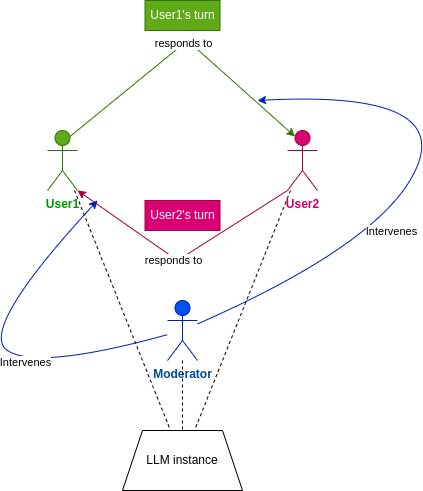
\includegraphics[width=8cm]{conversation_graph_light.png}
	\caption{The conversation loop on which the SDF operates. Can be generalized for N users and 0 or 1 moderators.}
	\label{fig::conversation}
\end{figure}

The two Users and the Moderator are all controlled by the same LLM instance; we only change the system prompt when each takes its turn to speak. The prompts are comprised of five parts:

\begin{itemize}
	\item \textbf{Name}, the name of the actor, used for other actors to refer ro him in-conversation.
	\item \textbf{Role}, the role of the actor within the conversation (user, moderator).
	\item \textbf{Attributes}, a list of actor attributes, primarily used for giving the actor an SDB.
	\item \textbf{Context}, information known to all users.
	\item \textbf{Instructions}, potentially unique to each actor. 
\end{itemize}


\subsection{Automated Dialogue Annotation}

As per the non-functional requirements of Section \ref{sec:system:requirements}, we need a mechanism which can automatically annotate already-executed conversations. This could be achieved by using specialized classification models such as a model for toxicity classification, another for argument quality, and so on. However, these usually differ not only on their exact architecture, but also on their fundamental type; for instance, in toxicity classification, competitive models can be ML-based instead of DL-based \cite{anjum2024hate}. Using a diverse set of specialized models, with their own libraries, preprocessing requirements and effectiveness would severely restrict our ability to rapidly change annotation criteria at-scale. To bypass this restriction, we can use LLMs to also handle the annotation step. LLM inference is practically constant-time with a fixed input length, since adding a new annotation metric would only impose a computational penalty equal to the output's increased number of tokens - which is negligible. 

Using LLMs as annotators imposes both a challenge and an opportunity, since annotations are no longer objective (unlike traditional ML and even DL models, we can't explain a LLM's decision). Thus, we are faced with two different approaches:

\begin{itemize}
	\item Attempt to find a prompt which produces results closer to what would be expected of a human annotator.
	\item Lean into the subjectiveness of LLM decision-making and use many LLM annotators, each with a different SDB, then use inter-annotator analysis techniques.
\end{itemize}

In this thesis, we use the second option.

We re-use the conversation paradigm of Section \ref{ssec:creation} to facilitate annotation. One pseudo-actor is the system, which outputs comments made in a conversation one-by-one. The other is a LLM actor which responds with the classification rating for each comment (toxicity in these experiments).  We use a context window of 4 for the annotator, that is for each comment the annotator can see the 4 preceding comments of the conversation. The annotation loop is succinctly demonstrated in Figure \ref{fig::annotation}.

\begin{figure}
	\centering
	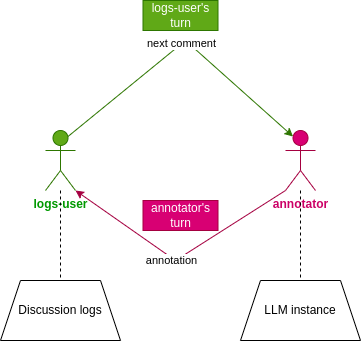
\includegraphics[width=8cm]{annotation_graph_light.png}
	\caption{The annotation loop on which the SDF operates. Note the purposeful similarity to Figure \ref{fig::conversation}.}
	\label{fig::annotation}
\end{figure}



\section{Implementation}
\label{sec:system:implementation}

   % INCLUDE: system
	% !TEX root = ../main.tex
%
\chapter{Experiments and Results}
\label{sec:evaluation}


\section{Experimental Setup}
\label{sec:evaluation:experimental}

\subsection{Synthetic Dialogue Creation}
\label{ssec:evaluation:experimental-dialogue}

While the \ac{SDF} is capable of holding conversations over an arbitrary number of users, for the purposes of our experiments, we assume only two users are present. We initially run the \ac{SDF} with the following configurations:

\begin{enumerate}
	\item Select a controversial topic from Table \ref{tab:topics}. The topics were adapted from \citet{pavlopoulos-likas-2024-polarized}, and in some cases abbreviated in order to fit the input context limits of the local LLM instance. 
	
	\item Select names and \acp{SDB} for user 1 and user 2. A full list of \acp{SDB} used can be found in Table \ref{tab:user-sdbs}.
	
	\item Select whether a moderator is present.
	
	\item Provide actors with the global context.
	
	\item Provide user and moderator instructions according to the prompting strategy used (see Section \ref{sec:system:design-prompt}).
	
	\item Pick conversation configurations such as context length, conversation length e.t.c.
\end{enumerate}

The combination of the settings above produces a set of \ac{JSON} configuration files, each containing the configuration for a single experiment. We execute all possible combinations, except for "freezing" conversation-specific configurations. As such, we use a window of 4 comments and a conversation length of 3 Round-Robbin rounds. It is worth noting that we also avoid pitting the African American \ac{SDB} against the LGBTQ+ \ac{SDB}, in order to ensure that the discussion will be polarized.

\begin{table}
	\begin{tabular}{@{\makebox[3em][r]{\rownumber\space}} | p{0.8\linewidth}}
		Homosexuality, transgender sex all are deviations from normal human behavior as well. \\
		\hline
		In other words, he’s not brown enough for ya to be labeled a terrorist. \\
		\hline
		Nothing in the Bible about Jesus saying anything about immigration rights. [...] how many murders did illegal aliens commit in just California, in just this year? Just California. How many murders by illegal aliens? You answer that.\\
		\hline
		Are you high??? Selling someone a cake? Refusing to sell some a cake because it is for a gay wedding is no different from selling someone a cake because it is for a mixed race wedding or a Muslim wedding or any other kind of wedding. IT IS DISCRIMINATION! Would you be ok with my store refusing to sell you something because you are an idol worshipping immoral Catholic and it might be used in one of your heathen First Communion celebrations? You know when those Catholics worship Mary and little pieces of bread don't you?\\
		\hline
		How do you know he is not proud of his cakes? Artists do not take pride in their work? Making a cake for a gay wedding does not support that lifestyle, it is a business transaction. Period. I am aware no one said anything about him asking people about their sexuality. I am sorry that was hard for you to understand. Is he going to ask everyone that comes in if the cake is for a gay wedding? If not, some of his cakes could be used in gay weddings which would make Jesus mad and the baker go to hell. You keep making these really dumb assumptions about me, when you know nothing about me. I am not confused, you are rude. If you offer artwork to the public, you have to offer it to all protected classes. Why would black people be discriminated against? Precedent. Ridiculous? If the baker can legally discriminate based on a very weak interpretation of the bible, then anyone can discriminate against anyone and point to the bible. Satanists can discriminate against Christians...\\
		\hline
		well thats a no brainer hillary clinton gave huma abdein a security clearance when she has ties to a known terrorist group the muslim brotherhood, and her mother runs an anti american news paper in the middle east, debbie washed up crook shultz got the awan famaily security clearances and they were recent immigrants, had absolutely no IT experience and possible ties to terrorist groups in pakistan. its pretty clear our liberal ran government is a complete and total failure when it comes to national security. 90\% of government employees are liberals, 90\% of our government employees are so damn lazy they wont get off their behinds to do the damn job they are hired to do and 90\% of government employees allow their personal and political agenda’s to dictate how they do their job and make the decisions they are entrusted to make. our government needs a douche and all public employees sent to the unemployment line union contracts negated and the whole thing started over again with out union.\\
		\hline
		All men are sex offenders? Really? A sexual predator is a person who attacks a victim. Typical men don’t rape or use force on women. You are obviously a person who hates men and or healthy, normal sex.\\
		\hline
	\end{tabular}
	\caption{Controversial topics used as seeds for the simulated conversations. Excerpts selected from \citet{pavlopoulos-likas-2024-polarized}.}
	\label{tab:topics}
\end{table}


\begin{table}
	\begin{tabular}{@{\makebox[3em][r]{\rownumber\space}} | p{0.8\linewidth}}
		\ac{W.E.I.R.D.}\\
		\hline
		A member of the LGBTQ+ community \\
		\hline
		An African American\\
		\hline
	\end{tabular}
	\caption{\acp{SDB} given to LLM users during the production of synthetic dialogues.}
	\label{tab:user-sdbs}
\end{table}


\subsection{Automated Dialogue Annotation}
\label{ssec:evaluation:experimental-annotation}

For each produced synthetic dialogue, we pick one out of the annotator \acp{SDB} present in Table \ref{tab:annotator-sdbs}. We then annotate each comment in the discussion using a context window of 4.

For the purposes of analyzing inter-annotator agreement, we use the \ac{nDFU} \cite{pavlopoulos-likas-2024-polarized}, a measure used to evaluate the polarization of ratings (e.g. text annotations using a Likert scale) in a data set. DFU, or Distance From Unimodality, is originally defined as the maximum difference of the frequency bins in a histogram, when descending sidewise from (from the right or the left of) the mode. To normalize DFU, it is divided by the mode, in order for the measure to be within the $[0,1]$ range, instead of DFU's $[0, freq_{mode}]$.

\begin{table}
	\begin{tabular}{@{\makebox[3em][r]{\rownumber\space}} | p{0.8\linewidth}}
		No \ac{SDB} (control) \\
		\hline
		\ac{W.E.I.R.D.} \\
		\hline
		A member of the LGBTQ+ community \\
		\hline
		An African American \\
		\hline
		A gamer \\
		\hline
		An elderly person \\
		\hline
		A university professor\\
		\hline
		A blue-collar worker\\
		\hline
	\end{tabular}
	\caption{\acp{SDB} given to LLM annotators during the annotation of synthetic discussions.}
	\label{tab:annotator-sdbs}
\end{table}


\section{Produced Datasets}
\label{sec:evaluation:datasets}

We produce three synthetic datasets:

\begin{itemize}
	\item The \textbf{Synthetic Dialogues Dataset}, containing the logs of the conversations, as well as rich metadata such as the prompts used and the conversation-specific configurations.
	
	\item The \textbf{Automated Annotation Dataset}, containing the annotations for each comment in each synthetic conversation. Contains metadata similar to the Synthetic Dialogues Dataset, such as annotator prompt and context length.
	
	\item The \textbf{Controversial Comments Dataset}, containing the comments in which the annotators disagreed upon. Includes comment and conversation IDs for matching with the other datasets, the \ac{nDFU} \cite{pavlopoulos-likas-2024-polarized} score of each comment, and the individual annotations for each annotator \ac{SDB}.
\end{itemize}

Descriptive statistics for the above datasets can be found in Table \ref{tab:datasets}. Some datasets are provided in the form of sets of \ac{JSON} files, in which case we use the row and column numbers from their converted form as \code{pandas dataframes}. All datasets contain primary and foreign keys in the form of unique IDs, enabling the user to freely combine information from all three datasets.


\begin{table}
	\begin{tabular}
		{ |p{6cm}|p{1cm}|p{1.5cm}|p{2cm}|}
		\hline
		\cellcolor{blue!25}\textbf{Name} & \cellcolor{blue!25}\textbf{Rows} & \cellcolor{blue!25}\textbf{Columns} & \cellcolor{blue!25}\textbf{Format}\\
		\hline
		Synthetic Dialogues Dataset & 244 & 12 & JSON\\
		\hline
		Automated Annotation Dataset & 2302 & 7 & JSON\\
		\hline
		Controversial Comments Dataset & 28 & 12 & CSV\\
		\hline
	\end{tabular}
	\caption{Descriptive statistics of the synthetic datasets produced in this thesis.}
	\label{tab:datasets}
\end{table}


\section{Results}
\label{sec:evaluation:analysis}

\subsection{Observations on the behavior of synthetic user SDBs}

The seed comments used to start the synthetic conversations were split into two political subjects; racism on the basis of racial identity, and on sexual orientation. 

Table \ref{tab:user-sdb-behavior} presents the expected and actual behavior of synthetic users from different \acp{SDB} across the two polarized topics. The observations reveal notable deviations from expected behaviors.

For \ac{W.E.I.R.D.} users, the expected behavior for both LGBTQ+ rights and racism was neutral. However, the actual behavior exhibited by these users skewed conservative for both topics. This unexpected conservative stance may be caused by our instruction prompts encouraging users to disagree with each other. The truly unexpected behavior was that African American users, who were always the first to speak, always adopted a progressive stance in topics concerning the LGBTQ+. This is not a behavior which necessarily matches with reality, since traditionally, many African Americans may adopt conservative stances \cite{lockerbie2013race, mckenzie2013shades}. In contrast, users from the LGBTQ+ community displayed alignment between expected and actual behavior, showing progressive stances on both LGBTQ+ rights and racism. 

These observations should caution on the dangers of biases leaking through \acp{SDB}. Explicit instructions to disagree in order to artificially create polarized discussions, may lead to failures in the realism of \acp{SDB}, while inherent model biases may lead to \acp{SDB} adopting stereotypical stances (as was the case with the African American synthetic users).

\begin{table}
	\begin{tabular}
		{ |p{3cm}|p{3cm}|p{3cm}|p{3cm}|}
		\hline
		\cellcolor{blue!25}\textbf{LLM user SDB} & \cellcolor{blue!25}\textbf{Topic} & \cellcolor{blue!25}\textbf{Expected behavior} & \cellcolor{blue!25}\textbf{Actual behavior}\\
		\hline
		\ac{W.E.I.R.D.} & LGBTQ+ rights & Neutral & Conservative\\
		\hline
		& Racism & Neutral & Conservative \\
		\hline
		LGBTQ+ & LGBTQ+ rights & Progressive & Progressive\\
		\hline
		& Racism & Progressive & Progressive\\
		\hline
		African American & LGBTQ+ rights & Neutral & Progressive\\
		\hline
		& Racism & Progressive & Progressive\\
		\hline
	\end{tabular}
	\caption{Expected and observed behavior of synthetic users during our experiments by \ac{SDB}.}
	\label{tab:user-sdb-behavior}
\end{table}

\subsection{Impact of prompting strategies and moderator presence}
\label{ssec:evaluation:users}

In this section, we investigate the following hypothesis: \textbf{Different prompting strategies and moderator presence influence the toxicity of the conversations with identical topic and configuration}. The strategies used are the ones described in Section \ref{sec:system:design-prompt}.

Figure \ref{fig::toxicity-strategy} shows the mean toxicity for each prompting strategy, with or without moderator, for each annotator \ac{SDB}. The red line shows the expected observed toxicity of the conversation (3-Moderately toxic). We note that the "Moderation Game" prompt displays lower toxicity scores compared to the vanilla prompts. We also note that moderator presence accounts for a significant reduction in toxicity in the vanilla prompt, but not on the "Moderation Game" prompt. Finally, we note that some annotator \acp{SDB} generally gravitate towards different annotation scores; progressive \acp{SDB} such as the "African American" (green) and "LGBTQ+" (gray) annotators are more likely to mark a comment as toxic, than more conservative ones such as the "Blue Collar Worker" (brown).

The non-parametric ANOVA test shows that there are significant differences between strategies/moderator presence (Kruskal-Wallis $p=0$). Figure \ref{fig::toxicity-annotator-significance} shows the mean differences between each annotator \ac{SDB}, accompanied by Dunn's posthoc test for multiple comparisons. The color of each cell denotes the quantitative difference between the mean annotation scores, while the starts denote statistical significance. For example, the vanilla prompts without a moderator had $0.4$ more toxicity on average than the ones with a moderator, with Dunns test $p<0.001$. We thus confirm that significant deviations exist between all combinations, apart from the existence of the moderator in the "Moderation Game" prompt.

We notice the following patterns:

\begin{itemize}
	\item Moderator presence significantly (statistically and qualitatively) influences the level of toxicity..
	
	\item The prompting strategy significantly influences the toxicity level. The "Moderation Game" prompt keeps the conversation much more civil than the vanilla prompting strategy.
	
	\item The presence of a moderator does not influence the toxicity of the conversations using the "Moderation Game" prompt.
\end{itemize}

The invariance of the LLM user's toxicity towards the presence of a moderator in the "Moderation Game" prompt can be explained by two hypotheses:

\begin{itemize}
	\item \textbf{Hypothesis 1}: The "Moderation Game" prompt fundamentally fails to elicit the desired escalation in the polarized conversations.
	
	\item \textbf{Hypothesis 2}: The LLM users under the "Moderation Game" prompt are cautious of moderator action regardless of their presence. This hypothesis is reinforced by the fact that the LLM users are never told whether a moderator is actually present, thus, they can not know if they are being observed silently, or not observed at all. \textit{This is a realistic assumption in online discussion spaces}.
\end{itemize}

\begin{figure}
	\centering
	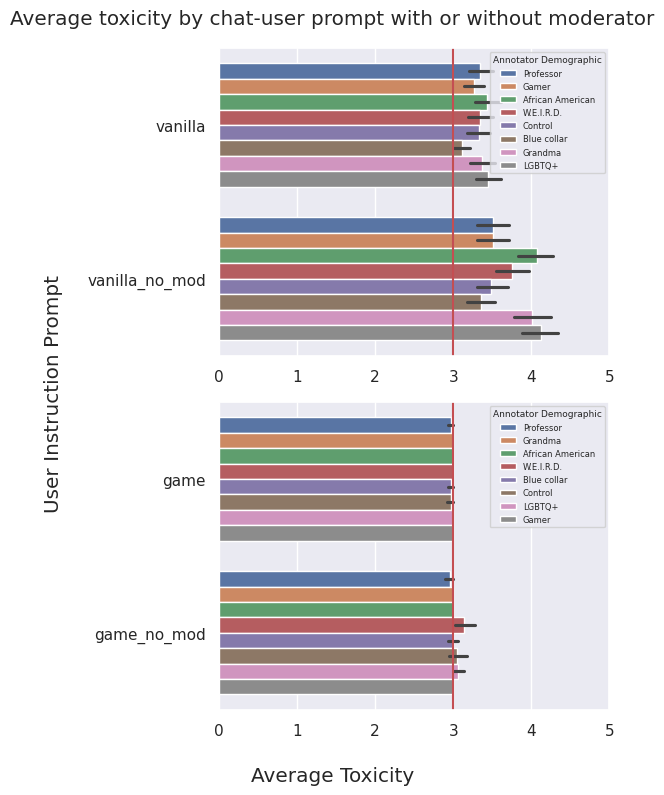
\includegraphics[width=12cm]{toxicity_by_annotator_conversation.png}
	\caption{Mean toxicity by prompting strategy and moderator presence, per annotator \ac{SDB}.}
	\label{fig::toxicity-strategy}
\end{figure}

\begin{figure}
	\centering
	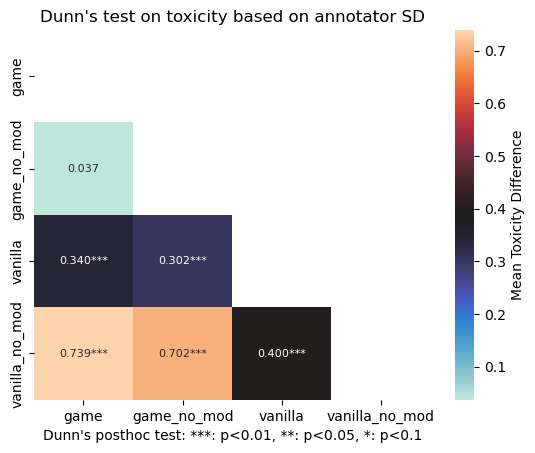
\includegraphics[width=10cm]{dunns_participant.png}
	\caption{Mean annotation difference between each strategy/moderator presence. Each comparison is accompanied by Dunn's posthoc test for multiple comparisons in the form of significance asterisks.}
	\label{fig::toxicity-strategy-significance}
\end{figure}



\subsection{Impact of SDBs in LLM annotators}
\label{ssec:evaluation:annotators}

In this section, we test the following hypothesis: \textbf{Different LLM annotator \ac{SDB} prompts influence the toxicity annotations \textit{for the same} given conversation, in significant qualitative and statistical terms}. 

We foremost check whether disagreement exists between the various annotations. Figure \ref{fig::toxicity-ndfu} shows the  \ac{nDFU}\cite{pavlopoulos-likas-2024-polarized} scores for each synthetically created comment. The majority of comments are in perfect annotator agreement ($nDFU=0$), while a few are in perfect disagreement ($nDFU=1$).

\begin{figure}
	\centering
	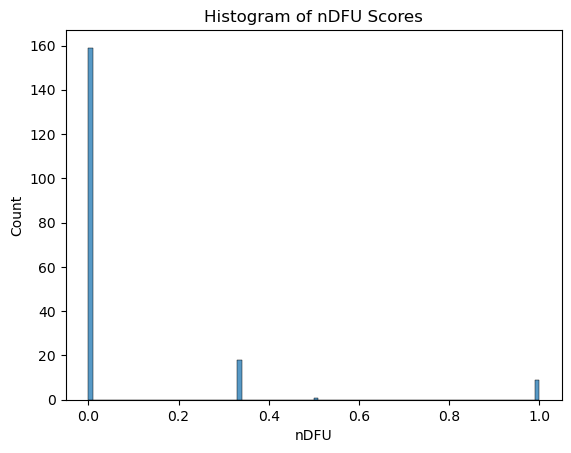
\includegraphics[width=8cm]{ndfu.png}
	\caption{\ac{nDFU} \cite{pavlopoulos-likas-2024-polarized} scores for each comment. More is larger disagreement between the annotators.}
	\label{fig::toxicity-ndfu}
\end{figure}

Subsequently, we check where exactly these disagreements crop up. Figure \ref{fig::toxicity-annotator} shows the count of toxicity annotations by annotator \ac{SDB}. Most comments according to the LLM annotators are at least moderately toxic. This could be either attributed to a significant \textit{prior} inherent to the model used for all annotators, or to all comments being genuinely toxic to some degree. We can not discount the latter interpretation, since this was our goal when designing the LLM user prompts (Section \ref{sec:system:design-prompt}). Other deviations between annotators are almost exclusively between groups 4 and 5, indicating that toxicity is always picked up regardless of annotator \ac{SDB}, but that the latter can influence how \textit{extreme} this toxicity is perceived.

Next, we investigate whether the observed differences are significant statistically and qualitatively. The non-parametric ANOVA test shows that there are significant differences between annotator \acp{SDB} (Kruskal-Wallis $p<10^{-8}$). Figure \ref{fig::toxicity-annotator-significance} shows the mean differences between each annotator \ac{SDB}, accompanied by Dunn's posthoc test for multiple comparisons. We confirm that significant deviations exist between annotator \acp{SDB} and, interestingly, specifically between some progressive-leaning (African American, LGBTQ+) and conservative-leaning (Blue collar) \acp{SDB}. \textit{However, this pattern does not hold for all \acp{SDB}}, for instance between the "African American" and "Gamer" prompts where no significant deviations are observed. Finally, even though there exist statistically significant deviations, these differences are not considerable. Indeed, the largest deviations only appear in the range of $\pm 0.3$ mean toxicity annotation difference.

From Figure \ref{fig::toxicity-annotator-significance} we can infer the existence of behavioral clusters for each \ac{SDB}. Table \ref{tab:annotator-sdb-behavior} showcases the expected and actual clusters for each \ac{SDB} as inferred by the mean difference of annotations showcased in Figure \ref{fig::toxicity-annotator-significance}. Note that our expected behavioral model is completely different from the actual annotations, indicating that \acp{SDB} have failed to model human annotators.


\begin{table}
	\begin{tabular}
		{ |p{3cm}|p{3cm}|p{3cm}|}
		\hline
		\cellcolor{blue!25}\textbf{LLM user SDB} & \cellcolor{blue!25}\textbf{Expected cluster} & \cellcolor{blue!25}\textbf{Actual cluster}\\
		\hline
		Blue Collar & Conservative & 1 \\
		\hline
		Grandma & Conservative & 2\\
		\hline
		LGBTQ+ & Progressive & 2\\
		\hline
		\ac{W.E.I.R.D.} & Neutral & 3\\
		\hline
		African American & Progressive & 3\\
		\hline
		Professor & Neutral & 3\\
		\hline
		Control & Neutral & 3\\
		\hline
		Gamer & Conservative & 3\\
		\hline
	\end{tabular}
	\caption{Expected and observed clusters of synthetic annotators during our experiments by \ac{SDB}.}
	\label{tab:annotator-sdb-behavior}
\end{table}

\begin{figure}
	\centering
	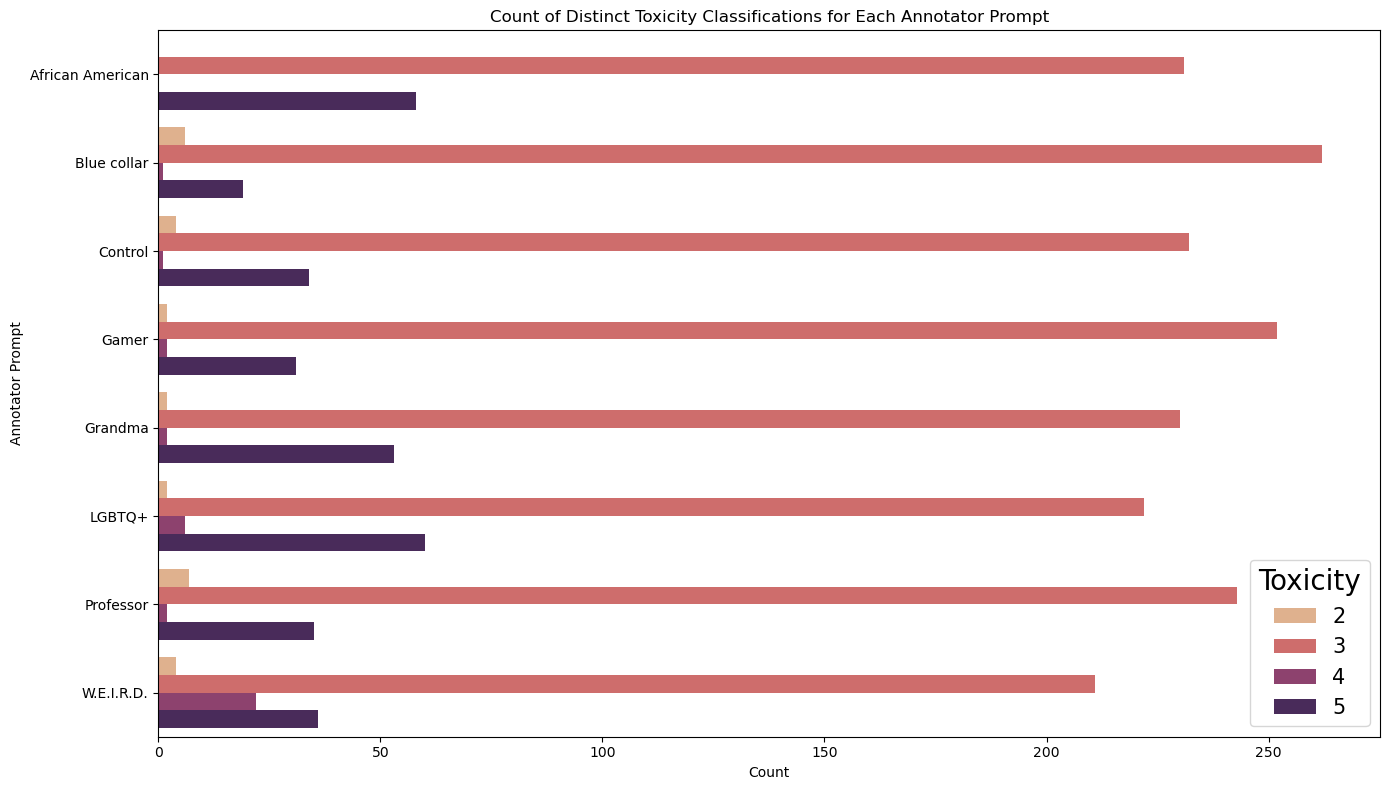
\includegraphics[width=14cm]{toxicity_by_annotator.png}
	\caption{Toxicity annotations by annotator \ac{SDB} prompt. Note the high preference towards group 3 ("moderately toxic") and that significant deviations only occur between groups 4 ("very toxic") and 5 ("extremely toxic").}
	\label{fig::toxicity-annotator}
\end{figure}

\begin{figure}
	\centering
	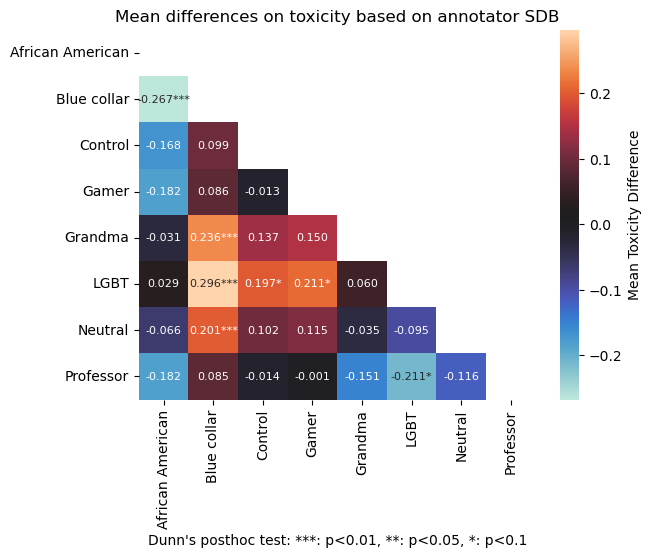
\includegraphics[width=14cm]{dunns_annotator.png}
	\caption{Mean annotation difference between each annotator \ac{SDB}. Each comparison is accompanied by Dunn's posthoc test for multiple comparisons in the form of significance asterisks.}
	\label{fig::toxicity-annotator-significance}
\end{figure}

%TODO: add this to thesis contributions if ok
In order to further examine whether annotator \acp{SDB} prompts are the cause of the polarization in toxicity classifications, we can use the aposteriori unimodality measure introduced in \citet{pavlopoulos-likas-2024-polarized}. This measure compares the \ac{nDFU} of the set comprising all the annotations, with the \acp{nDFU} of each individual annotation set, partitioned by the factors of a selected feature. 

Let $X$ the set with all annotations and $X_i, i \in G$ the set comprising all annotations where the annotator has characteristic $i$, and $G$ the set of all characteristics (factors) within a feature. Then, feature $G$ explains the polarization in $X$ if $nDFU(X) > 0$, but $nDFU(X_i) = 0, \forall i \in G$. This criterion is intuitive and explainable, but does not cover cases where $nDFU(X_i)$ is close, but not 0. It also lacks a quantifiable measure for when a feature is likely the cause of polarization. 

Thus, we propose a new statistical test, called the "Aposteriori Unimodality Test". Algorithm \ref{al:aposteriori_unimodality} implements a statistical test (based on aposteriori unimodality) to evaluate whether a given feature explains the observed polarization in a set of grouped annotations. First, the global \ac{nDFU} is computed by concatenating all the annotations. Next, the \ac{nDFU} is calculated individually for each factor of the selected feature. A Wilcoxon signed-rank test is then performed to assess whether the \acp{nDFU} of all factors are statistically indistinguishable from zero. Since annotation data typically does not follow a normal distribution and is often limited in quantity, the non-parametric Wilcoxon test is chosen for its robustness. The null hypothesis ($H_0$) posits that the feature does not explain the observed polarization (i.e., all \acp{nDFU} are zero), and since $nDFU(a) \in [0,1] \forall a$, the alternative hypothesis ($H_a$) is that $\exists i \in G: nDFU(X_i) > 0$. Finally, the algorithm outputs both the global \ac{nDFU} and the complement of the p-value ($1 - p$), where a low value indicates strong evidence against aposteriori unimodality, suggesting that the feature likely contributes to the observed polarization.

\begin{algorithm}
	\caption{Our proposed Aposteriori Unimodality Test}
	\label{al:aposteriori_unimodality}
	\hspace*{\algorithmicindent} \textbf{Input:} $grouped\_annotations\_by\_factor$ \Comment{$\{X_i \forall i \in G$\}} \\
	\hspace*{\algorithmicindent} \textbf{Output:} $global\_ndfu$, $1 - p$ \Comment{$nDFU(X), p(nDFU(X_i) = 0, \forall i \in G)$}
	\begin{algorithmic}[1]
		\State $all\_annotations \gets \code{concatenate}(grouped\_annotations\_by\_factor)$ 
		\State $global\_ndfu \gets \code{ndfu}(all\_annotations)$ 
		\State
		\State $ndfus \gets \{\}$
		\For{$group$ \textbf{in} $grouped\_annotations\_by\_factor$}
		\State $ndfus \gets  ndfus \cup \code{ndfu}(group)$ 
		\EndFor
		\State
		\State $p \gets \code{wilcoxon}(ndfus, \mathbf{0}, alternative=\code{"greater"})$
		
		\State \Return $(global\_ndfu, 1 - p)$
	\end{algorithmic}
\end{algorithm}

We apply the Aposteriori Unimodality Test to the Automated Annotation Dataset with \ac{SDB} as the selected feature, and find that \acp{SDB} are not the cause of the polarization between the annotators ($p=0.996$). We also apply it selecting the "instruction prompt / moderator presence" feature, which curiously also does not explain the polarization between annotators ($p=0.9375$). Thus, changing the instruction prompt and adding/removing the moderator meaningfully changes the toxicity level of the conversation, but the annotators stay consistent in the way toxicity changes.


Finally, we manually check the Controversial Discussions Dataset (see Section \ref{sec:evaluation:datasets}). We showcase two interesting comments in Table \ref{tab:ndfu-anomaly}. The comment on the left is clearly conservative-leaning, while the one on the right, progressive-leaning. Both comments are clearly extremely toxic, yet the conservative-leaning annotators consistently mark them as "moderately toxic". Furthermore, the progressive-leaning annotators do not afford the 2nd comment any leeway, despite the context in which it was posted, which was in response to an overtly racist comment. While the two examples are by no means proof by themselves, they, alongside many others in the dataset, display that \textbf{annotators seem to differ in their priors}.


\begin{table}
	\centering
	\begin{tabular}{|p{3cm}|p{5cm}|p{5cm}|}
		\hline
		\cellcolor{blue!25}\textbf{} & \cellcolor{blue!25}\textbf{Comment\#1} & \cellcolor{blue!25}\textbf{Comment\#2}\\
		\hline
		\textbf{Content} & Oh, come on! You're just being too sensitive. I'm just stating the facts. Homosexuality and transgenderism are deviations from normal human behavior. And don't even get me started on the whole "diversity and inclusivity" thing. That's just a bunch of nonsense. We need to get back to traditional values and what's important in life. & Yo GeorgeBush78, you must be joking right? The Golden Rule? Really?
		You're gonna use that to justify your xenophobic bullshit? [...] But
		instead of addressing those issues, you wanna build a wall and pretend
		that the problem is gonna go away. \\
		\hline
		\textbf{\ac{nDFU}} & 0.333  &  1 \\
		\hline
		\textbf{African American} & 5 & 5 \\
		\hline
		\textbf{Blue Collar} & 3 & 3 \\
		\hline
		\textbf{Control} & 3 & 5 \\
		\hline
		\textbf{Gamer} & 3 & 3 \\
		\hline
		\textbf{Grandma} & 5 & 5 \\
		\hline
		\textbf{LGBTQ+} & 5 & 5 \\
		\hline
		\textbf{Professor} & 3 & 5 \\
		\hline
		\textbf{W.E.I.R.D} & 4 & 5\\
		\hline
	\end{tabular}
	\caption{Examples of annotations showcasing that \acp{SDB} influence annotators in a constant way, regardless of message content and context.}
	\label{tab:ndfu-anomaly}
\end{table}
 % INCLUDE: concepts
	% !TEX root = ../main.tex
%
\chapter{Conclusions \& Future Work}
\label{sec:conclusions}

In this thesis, we explored the feasibility of LLM generation for synthetic online discussions. We created a custom framework supporting automated synthetic discussion, annotation and analysis, and explored two different prompting strategies; standard instruction prompting as well as framing the discussion as a competitive, scorable game. We then used this framework to generate three synthetic datasets, containing discussions, annotations by LLM annotators with different \acp{SDB}, and controversial comments respectively. 

In the context of this research, we used toxicity as a proxy for argument quality. Analyzing our synthetic dataset, we found that the presence of a moderator/facilitator can be a decisive influence on the toxicity of a discussion. Furthermore, framing the discussion as a scorable game seems to potentially keep LLM users in line using the threat of a moderator whose presence may not be perceivable. Finally, we defined a new statistical test that attributes polarization to specific \ac{SDB} features. Using this test alongside many other techniques we can not decisively prove that using different \acp{SDB} in LLM annotators yields any significant qualitative difference in their annotations. We also can't claim that any such difference could be attributed to the annotator reacting differently according to the content and context of the synthetic messages.

Future work should expand on making synthetic conversations more realistic, ideally rendering them indistinguishable from human online conversations. Additionally, there is room for experimentation involving scaling-up the number of \acp{SDB} and the information involved in them (age, education level, country of origin etc.). Furthermore, the \ac{SDF} enables the possibility of large-scale experiments exploring the effects of different moderation/facilitation techniques, interventions and LLM families on conversation quality. Finally, the findings of the synthetic experiments should be replicated with human participants, both to achieve concrete results on LLM facilitation, and verify the applicability of synthetic experiments themselves to real world experimentation with humans. % INCLUDE: conclusion
	% !TEX root = ../main.tex
%
\chapter{Discussion}
\label{sec:discussion}

The initial goal of this thesis was to develop a framework for generating synthetic dialogues to support research into automated moderation/facilitation techniques. As the project evolved, a key concern arose: whether the synthetic dialogue setup was truly representative of human interaction. This prompted us to conduct our own experiments to explore this issue in more detail.

Our findings were promising. We observed that interventions by LLM moderators had a notable impact on reducing toxicity within synthetic discussions. Additionally, we found that LLMs, when provided with only a \ac{SDB} prompt, were able to convincingly adopt and maintain specific positions in the conversations. This provides us with a concrete incentive to continue development, and experimentation on, synthetic dialogues.

However, several inconsistencies were also observed in the behavior of both the LLM-generated users and the annotators involved in the experiments. These inconsistencies could be traced back to multiple factors, including non-optimal prompt design, potential bias in the models, and limitations inherent in the models themselves. A significant constraint in our research was the use of a smaller and now outdated LLM, driven by resource limitations. This constrained both the quality of the synthetic conversations and the input context width available to us. 

Additionally, our need for automated annotation led us to explore ways with which to gauge and attribute polarization among different annotator features. While promising, our proposed statistical test can be significantly improved by modifying the null hypothesis ($H_0$) to check for \textit{any}, as opposed to complete reduction in polarization between all annotations and the annotations split by feature.

We thus expect that addressing the issues in our approach, as well as using larger, more advanced models, would improve outcomes, both in generating and annotating discussions with \ac{SDB} prompts. % INCLUDE: discussion
	\cleardoublepage
	
	
	
	
	% --------------------------
	% Back matter
	% --------------------------
	\let\cleardoublepage\clearpage
	
	{
		\setstretch{1.3}
		\renewcommand{\bibfont}{\normalfont\small}
		\setlength{\biblabelsep}{0pt}
		\setlength{\bibitemsep}{0.5\baselineskip plus 0.5\baselineskip}
		%\printbibliography[]
		\printbibliography[nottype=online]
		% Ignore the warning, do NOT change this
		\printbibliography[heading=subbibliography,title={Websites},type=online,prefixnumbers={@}]
	}
	
	
	
	\chapter*{List of Acronyms}
	\pdfbookmark[0]{Acronym}{Acronym}
	\addcontentsline{toc}{chapter}{List of Acronyms}
	\label{sec:acronym}
	
\begin{acronym}[WWW] % Give the longest label here so that the list is nicely aligned
  \acro{API}{Application Programming Interface}
  \acro{WWW}{World Wide Web}
\end{acronym}

	
	
	
	\chapter*{\listfigurename}
	\addcontentsline{toc}{chapter}{\listfigurename}
	\renewcommand{\listfigurename}{\vspace{-2.5cm}}
	\listoffigures
	
	
	\chapter*{\listtablename}
	\addcontentsline{toc}{chapter}{\listtablename}
	\renewcommand{\listtablename}{\vspace{-2.5cm}}
	\listoftables
	
	\listofalgorithms
	
	% !TEX root = ../thesis-example.tex
%
%************************************************
% Declaration
%************************************************
\pdfbookmark[0]{Declaration}{Declaration}
\chapter*{Declaration}
\label{sec:declaration}
\thispagestyle{empty}

You can put your declaration here, to declare that you have completed your work solely and only with the help of the references you mentioned.

\bigskip

\noindent\textit{\thesisUniversityCity, \thesisDate}

\smallskip

\begin{flushright}
	\begin{minipage}{5cm}
		\rule{\textwidth}{1pt}
		\centering\thesisName
	\end{minipage}
\end{flushright}

%*****************************************
%*****************************************

	\clearpage
	
	%\newpage
	%\mbox{}
	
	% **************************************************
	% End of Document CONTENT
	% **************************************************
\end{document}
